\subsection{Debugging-Profiling-Optimization-Parallelization}

\begin{frame}[containsverbatim]
	\frametitle{SDLC}
%	\begin{figure}[ht!]
%	\centering
	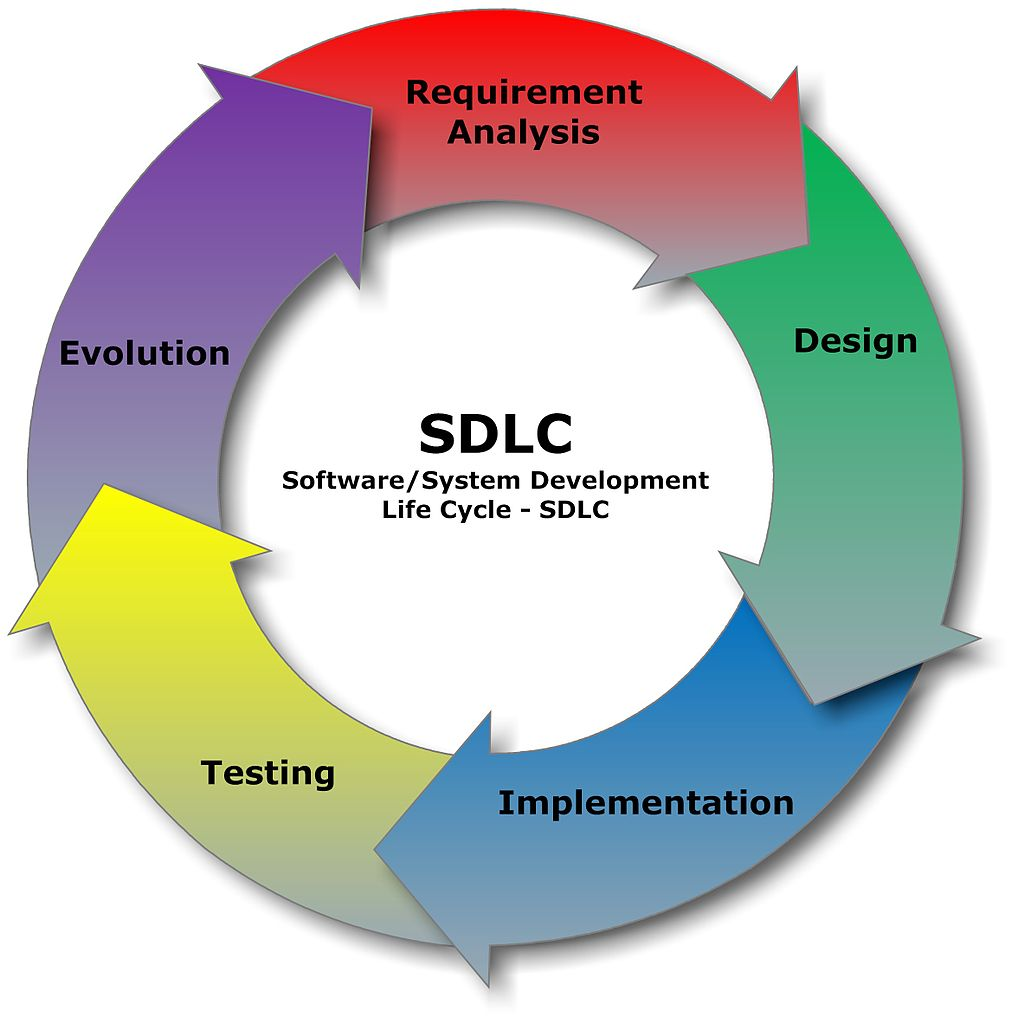
\includegraphics[width=85mm]{Day1/images/SDLC.jpg}
%	\end{figure}
\end{frame}



\begin{frame}
	\frametitle{Before you start your parallel implementation}

	\begin{itemize}
	\item {\bf You have no serial code : } design your application in a parallel way from scratch
	\item {\bf You have a serial code :} follow a Debugging-Profiling-Optimization cycle before any parallelization
	\end{itemize}
\end{frame}

\subsubsection{Debugging}

\begin{frame}
	\frametitle{Debugging ?}

	\begin{itemize}
	\item Find and correct bugs within an application
	\item Bugs can be of various nature : division by zero, buffer overflow, null pointer, infinite loops, etc.. 
	\item The compiler is (very) rarely able to recognize a bug at compilation time and the error is (very) rarely explicit regarding the bug ("syntax error")
	\item Use standard tools like {\tt gdb} 
	\item A multi-threaded code can be tricky to debug (race conditions, deadlocks, etc..)
	\item (Complex) tools exist for parallel debug : {\tt Totalview}, {\tt Alinea DDT} or recently {\tt Eclipse PTP}
	\end{itemize}

\end{frame}


\subsubsection{Profiling}

\begin{frame}
	\frametitle{Profiling ?}

Where do I spend most of the time ? 

	\begin{itemize}
	\item (good) using tools like {\tt gprof} or {\tt Intel Amplifier}
	\item (bad) ``by hand'' using timings and {\tt printf}'s
	\end{itemize}
\end{frame}

\begin{frame}
	\frametitle{Profiling ?}

What should be profiled ?

	\begin{itemize}
	\item TTS (Time To Solution)
	\item best usage of resources (storage, memory, etc..)
	\item behavior of the application to scale
	\item ...
	\end{itemize}
\end{frame}



\begin{frame}[containsverbatim]
	\frametitle{Profiling : an example with gprof}

	\begin{itemize}
	\item {{\bf MiniFE as test application} 
		\begin{itemize}
			\item 3D implicit finite-elements on an unstructured mesh
			\item mini-application written in C++
			\item \url{http://www.mantevo.org}
		\end{itemize}
	}
	\item compile with {\tt -pg -g -O3 -ftree-vectorize}
	\item run it. It should produce a {\tt gmon.out} file
	\item then profile it {\tt gprof miniFE.x}
	\end{itemize}
\end{frame}


\begin{frame}[containsverbatim]
	\frametitle{Profiling : an example with gprof}

Size : ($128~x~128~x~128$)

	\begin{Verbatim}[fontsize=\tiny]
Flat profile:

Each sample counts as 0.01 seconds.
  %   cumulative   self              self     total           
 time   seconds   seconds    calls   s/call   s/call  name    
 62.15      2.61     2.61        1     2.61     2.61  void miniFE::cg_solve
  8.57      2.97     0.36        2     0.18     0.18  void miniFE::impose_dirichlet
  5.71      3.21     0.24  7471812     0.00     0.00  int miniFE::find_row_for_id
  5.71      3.45     0.24   274625     0.00     0.00  void miniFE::Hex8::diffusionMatrix_symm
  4.76      3.65     0.20   274625     0.00     0.00  void miniFE::sum_in_symm_elem_matrix
  2.62      3.76     0.11  2197000     0.00     0.00  void miniFE::Hex8::gradients_and_invJ_and_detJ
  1.90      3.84     0.08   274625     0.00     0.00  void miniFE::get_elem_nodes_and_coords
  1.90      3.92     0.08        1     0.08     0.08  int miniFE::verify_solution
  1.67      3.99     0.07  2197000     0.00     0.00  void miniFE::Hex8::gradients_and_detJ
  0.95      4.03     0.04   274625     0.00     0.00  void miniFE::Hex8::sourceVector
  0.95      4.07     0.04        1     0.04     0.04  void miniFE::make_local_matrix
  0.71      4.10     0.03        1     0.03     0.03  std::vector::_M_fill_insert
  0.71      4.13     0.03  1649773     0.00     0.00  miniFE::mytimer()
  0.71      4.16     0.03        1     0.03     0.31  int miniFE::generate_matrix_structure
  0.48      4.18     0.02        1     0.02     0.03  void miniFE::create_map_id_to_row
  0.24      4.19     0.01        8     0.00     0.00  void miniFE::get_ids
  0.24      4.20     0.01        1     0.01     0.27  void miniFE::init_matrix
  0.00      4.20     0.00   270400     0.00     0.00  void sort_if_needed
  0.00      4.20     0.00    33282     0.00     0.00  std::_Rb_tree

...
	\end{Verbatim}
\end{frame}


\begin{frame}
	\frametitle{Profiling : an example with gprof}

What do we learn ?

	\begin{itemize}
	\item 62.15 \% of the time is spent in the solver (Conjugate Gradient)
	\item 8.57 \% is spent in imposing the boundary conditions
	\item etc..
	\item with that specific problem size ($128~x~128~x~128$). Is that similar with a larger/smaller one ?
	\end{itemize}
\end{frame}


\begin{frame}[containsverbatim]
	\frametitle{Profiling : an example with gprof}

Smaller ($16~x~16~x~16$)

	\begin{Verbatim}[fontsize=\tiny]
Flat profile:

Each sample counts as 0.01 seconds.
  %   cumulative   self              self     total           
 time   seconds   seconds    calls  ms/call  ms/call  name    
100.01      0.01     0.01        1    10.00    10.00  void miniFE::cg_solve
  0.00      0.01     0.00    18605     0.00     0.00  int miniFE::find_row_for_id
  0.00      0.01     0.00     5832     0.00     0.00  void miniFE::Hex8::gradients_and_detJ
  0.00      0.01     0.00     5832     0.00     0.00  void miniFE::Hex8::gradients_and_invJ_and_detJ
  0.00      0.01     0.00     4907     0.00     0.00  miniFE::mytimer()
  0.00      0.01     0.00      729     0.00     0.00  void sort_if_needed
  0.00      0.01     0.00      729     0.00     0.00  void miniFE::sum_in_symm_elem_matrix
  0.00      0.01     0.00      729     0.00     0.00  void miniFE::get_elem_nodes_and_coords
  0.00      0.01     0.00      729     0.00     0.00  void miniFE::Hex8::sourceVector<double>
  0.00      0.01     0.00      729     0.00     0.00  void miniFE::Hex8::diffusionMatrix_symm
  0.00      0.01     0.00      578     0.00     0.00  std::_Rb_tree<int, std::pair
  0.00      0.01     0.00      300     0.00     0.00  std::_Rb_tree<int, int, std::_Identity
  0.00      0.01     0.00      271     0.00     0.00  std::_Rb_tree<int, std::pair
  0.00      0.01     0.00      153     0.00     0.00  add_timestring_to_yaml
  0.00      0.01     0.00       52     0.00     0.00  void miniFE::exchange_externals
  0.00      0.01     0.00       26     0.00     0.00  std::vector<int, std::allocator
  0.00      0.01     0.00       25     0.00     0.00  miniFE::TypeTraits<miniFE::Vector

...
	\end{Verbatim}
\end{frame}


\begin{frame}[containsverbatim]
	\frametitle{Profiling : an example with gprof}

Larger ($512~x~512~x~512$)

	\begin{Verbatim}[fontsize=\tiny]
Flat profile:

Each sample counts as 0.01 seconds.
  %   cumulative   self              self     total           
 time   seconds   seconds    calls   s/call   s/call  name    
 63.70    228.52   228.52        1   228.52   228.87  void miniFE::cg_solve
 11.96    271.43    42.91 471862020     0.00     0.00  int miniFE::find_row_for_id
  4.87    288.90    17.47        2     8.74     8.74  void miniFE::impose_dirichlet
  4.04    303.38    14.48 16974593     0.00     0.00  void miniFE::Hex8::diffusionMatrix_symm
  3.48    315.87    12.49 16974593     0.00     0.00  void miniFE::sum_in_symm_elem_matrix
  3.29    327.68    11.81 16974593     0.00     0.00  void miniFE::get_elem_nodes_and_coords
  1.96    334.72     7.04 135796744     0.00     0.00  void miniFE::Hex8::gradients_and_invJ_and_detJ
  1.74    340.96     6.24        1     6.24     6.24  int miniFE::verify_solution
  1.29    345.60     4.64 135796744     0.00     0.00  void miniFE::Hex8::gradients_and_detJ
  0.82    348.54     2.94 16974593     0.00     0.00  void miniFE::Hex8::sourceVector
  0.64    350.83     2.29        1     2.29    45.48  void miniFE::init_matrix
  0.43    352.36     1.53        1     1.53     1.53  std::vector
  0.42    353.88     1.52        1     1.52     1.70  void miniFE::make_local_matrix
  0.40    355.31     1.43        1     1.43    48.45  int miniFE::generate_matrix_structure
  0.35    356.55     1.24 101849581     0.00     0.00  miniFE::mytimer()
  0.16    357.14     0.59        1     0.59    55.23  void miniFE::perform_element_loop
  0.11    357.55     0.41        8     0.05     0.05  void miniFE::get_ids
  0.09    357.88     0.33      201     0.00     0.00  void miniFE::exchange_externals
  0.08    358.18     0.30 16908544     0.00     0.00  void sort_if_needed
  0.05    358.35     0.17        1     0.17     0.66  void miniFE::create_map_id_to_row

...
	\end{Verbatim}
\end{frame}

\begin{frame}
	\frametitle{Profiling : an example with gprof}

Some tricks

	\begin{itemize}
	\item profile a code {\bf without bugs}
	\item choose the right size of the problem to profile (not too small, not too large)
	\item concentrate the optimization phase to the most consuming parts
	\item if the profile is not explicit, try to split the code by refactoring it into smaller functions calls
	\item take a tour of the different {\tt gprof} options
	\item {\tt gprof} works with parallel codes (OpenMP, MPI, hybrid)
	\end{itemize}
\end{frame}

\begin{frame}[containsverbatim]
	\frametitle{Profiling : with Intel Amplifier (General)}
%	\begin{figure}[ht!]
%	\centering
	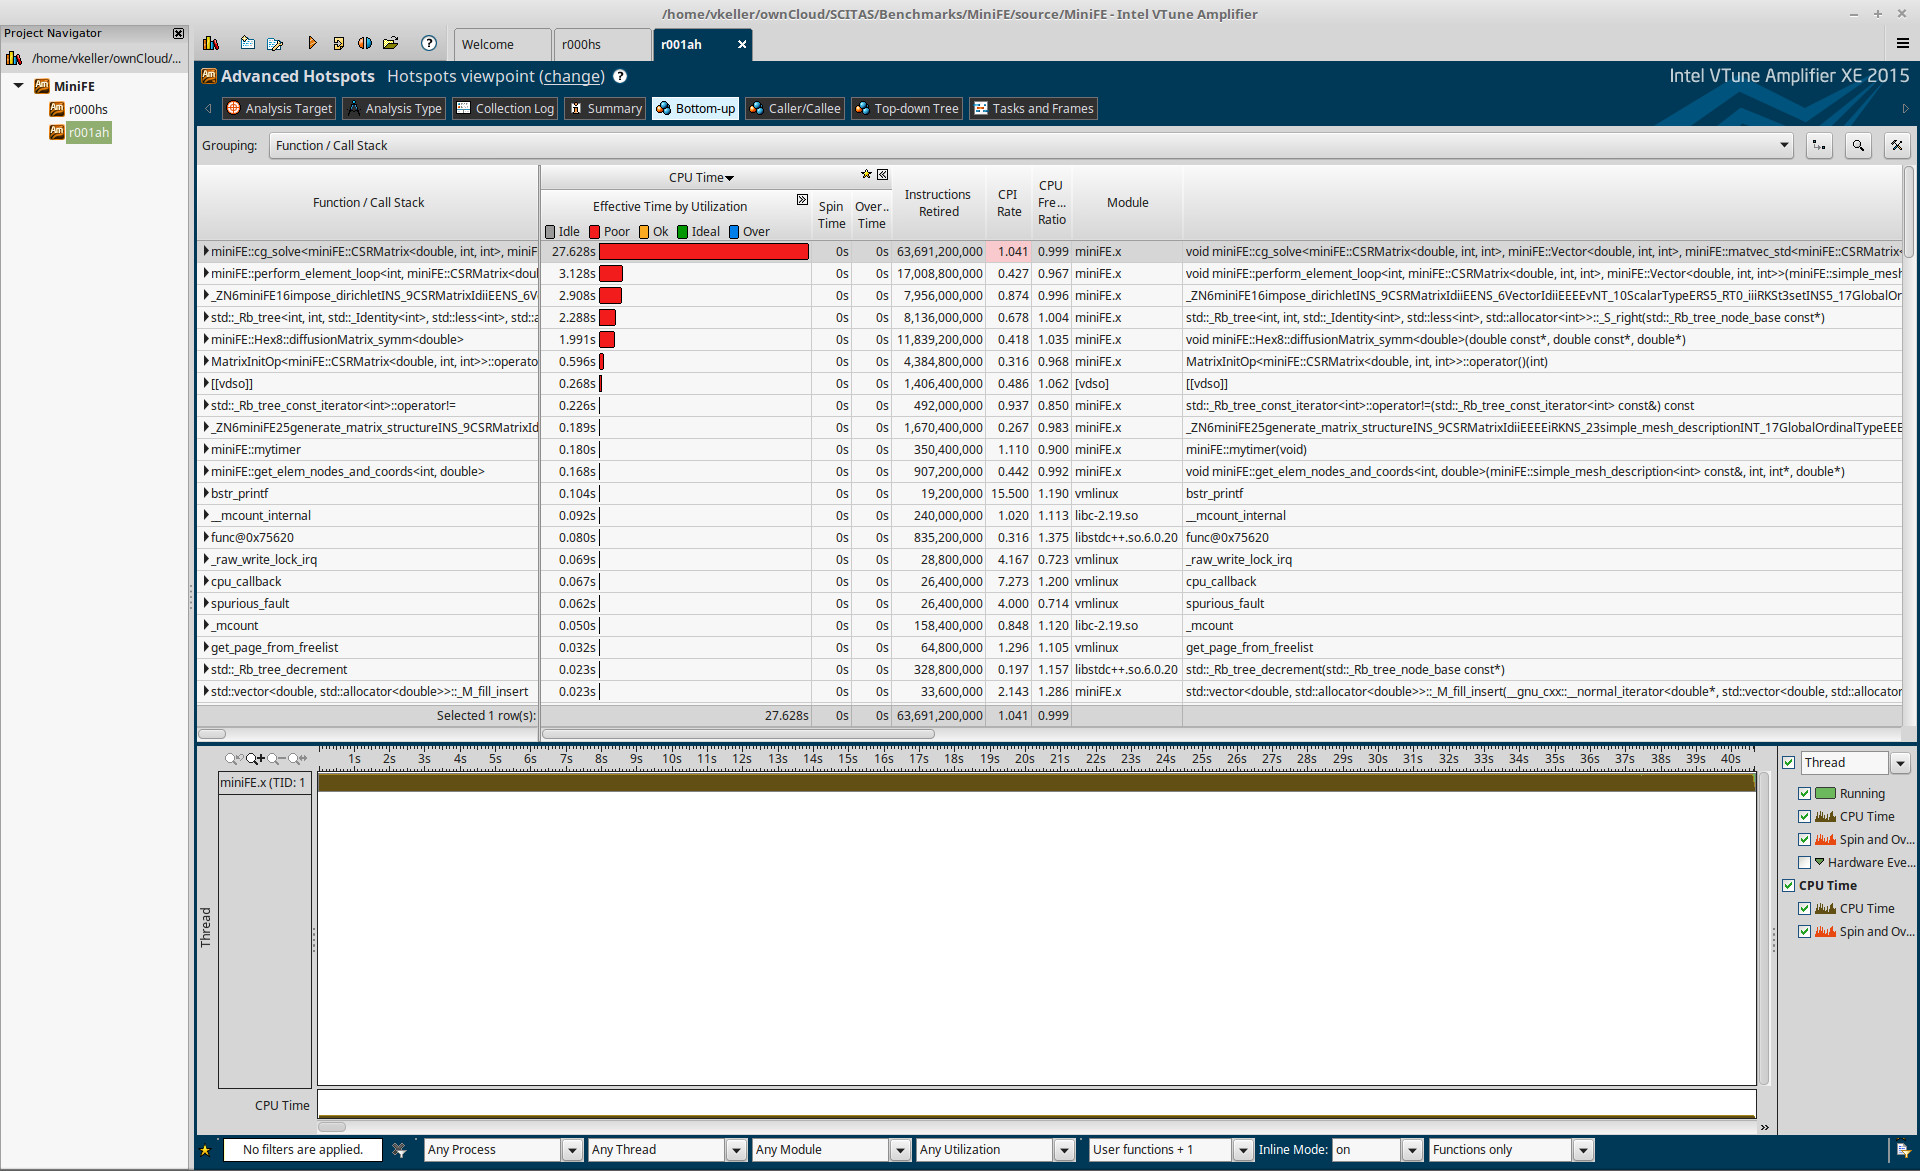
\includegraphics[width=115mm]{Day1/images/Amplifier1.jpg}
%	\end{figure}
\end{frame}

\begin{frame}[containsverbatim]
	\frametitle{Profiling : with Intel Amplifier (HW counters)}
%	\begin{figure}[ht!]
%	\centering
	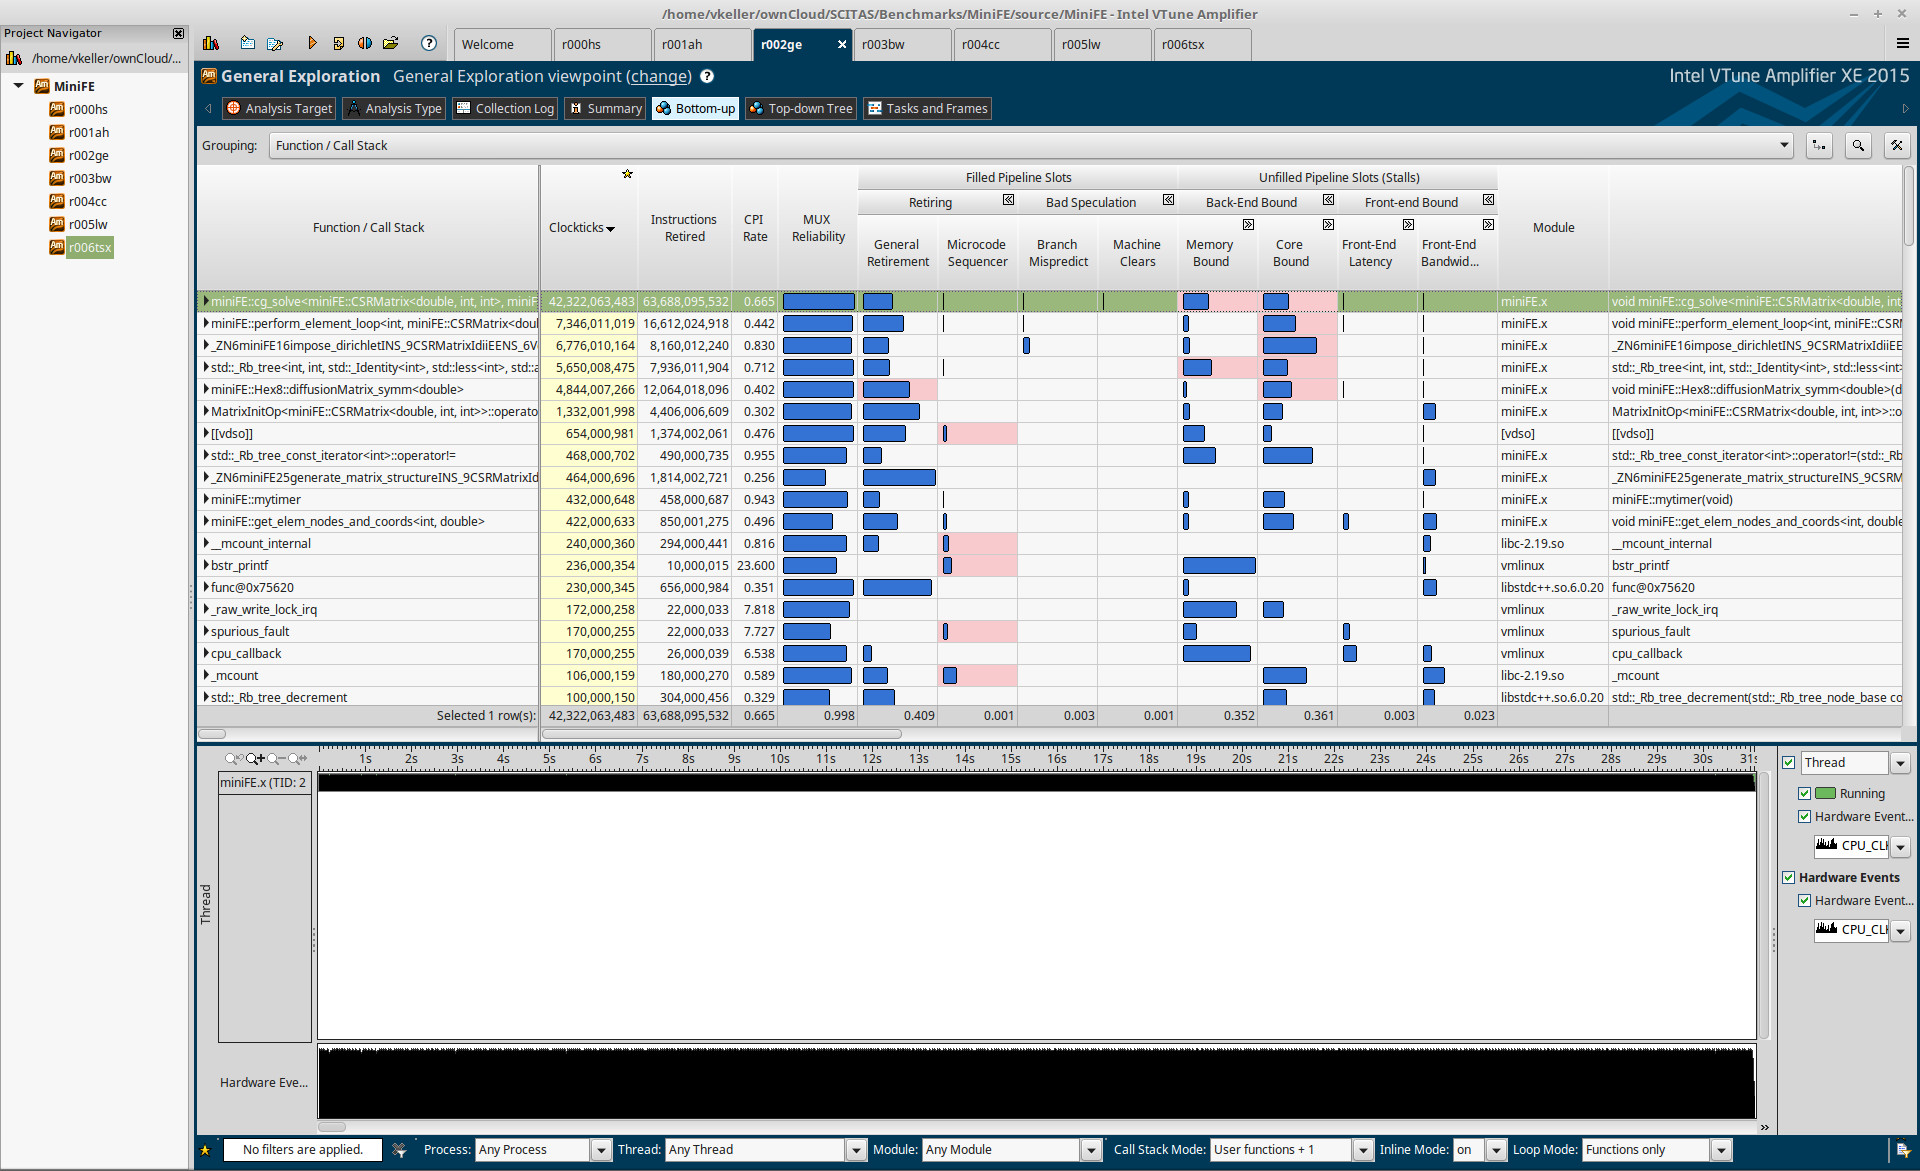
\includegraphics[width=115mm]{Day1/images/Amplifier2.jpg}
%	\end{figure}
\end{frame}

\begin{frame}[containsverbatim]
	\frametitle{Profiling : with Intel Amplifier (Bandwidth)}
%	\begin{figure}[ht!]
%	\centering
	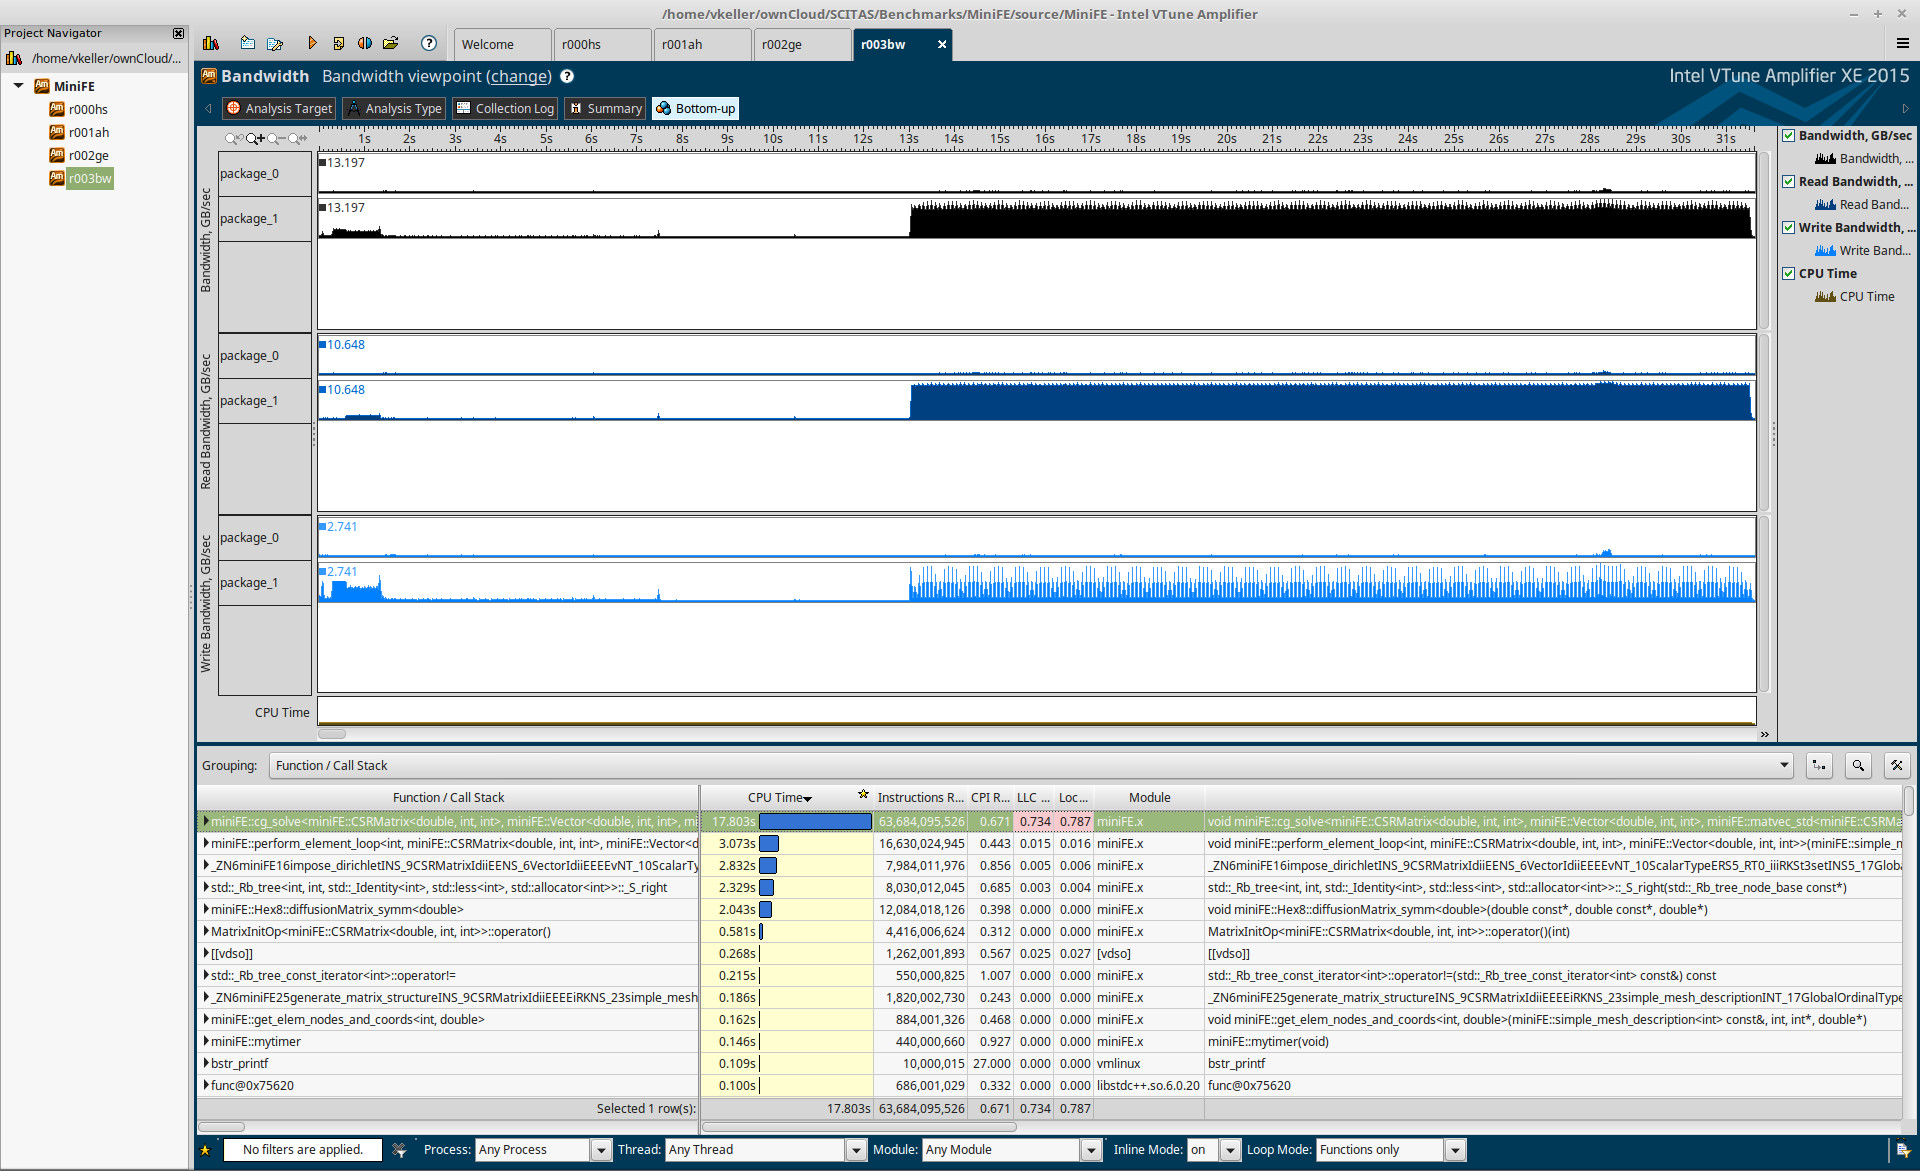
\includegraphics[width=115mm]{Day1/images/Amplifier3.jpg}
%	\end{figure}
\end{frame}

\begin{frame}
	\frametitle{Profiling : with Intel Amplifier}

What do we learn ?

	\begin{itemize}
	\item the Conjugate Gradient solver ({\tt cg$\_$solve}) is the most consuming part
	\item this is due to the memory bandwidth (read from memory) limit (measured : 10.65 GB/s peak : 17.1 GB/s = DDR4-2133, STREAM : 11.8 GB/s)
	\item CPI (Clockticks per Instructions Retired) is good (0.65) : the latency is {\it probably} not a problem (cache misses, I/O or other bottlenecks)
	\end{itemize}
\end{frame}

\subsubsection{Optimization}

\begin{frame}
	\frametitle{Optimization ?}

	By order of complexity :

	\begin{enumerate}
	\item compiler and linker flags
	\item optimized external libraries
	\item ``handmade'' refactoring (loop reordering, usage of intrinsics, memory alignment, etc.. )
	\item algorithmic changes
	\end{enumerate}
\end{frame}

%\begin{frame}
%	\frametitle{Optimization : how to compare ?}
%
%	\begin{itemize}
%	\item 
%	\item 
%	\item 
%	\end{itemize}
%
%\end{frame}

\begin{frame}
	\frametitle{Optimization : when to stop ?}

Empirical ''80-20 law'' or ''The Pareto law'' : roughly 80 \% of the time is spent in 20 \% of the code

	\begin{itemize}
	\item concentrate on these 20 \% of the code
	\end{itemize}

Example with MiniFE : 80 \% of the time is spent in the solver (63), the boundary conditions (8) and reordering (5).

\end{frame}



\subsubsection{Parallelization}

\begin{frame}
	\frametitle{Parallelization ?}

Only when your sequential code has {\bf no bug} and is {\bf optimized}.

	\begin{enumerate}
	\item Is it worth to parallelize my code ? Does my algorithm scale ?
	\item Performance prediction ?
	\item Timing diagram ?
	\item Bottlenecks ? 
	\item Which parallel paradigm should I chose ? What is the target architecture (SMP, cluster, GPU, hybrid, etc..) ? 
	\end{enumerate}
\end{frame}




\subsection{A few words on high performance}


\begin{frame}
\frametitle{Parallelization of an unoptimized code}
%\framesubtitle{(... or parallelization of a non-appropriate algorithm)}

\begin{columns}
%\begin{column}[l]{7cm}
\begin{column}{7cm}
Back in 1991, David H. Bailey from Lawrence Berkeley National Laboratory released a famous paper in the Supercomputing Review: \textit{``Twelve Ways to Fool the Masses When Giving Performance Results on Parallel Computers''}.

\begin{block}{}
Number 6 was: \textit{Compare your results against scalar, unoptimized code on Crays.}
\end{block}

\end{column}
\begin{column}[c]{3cm}
{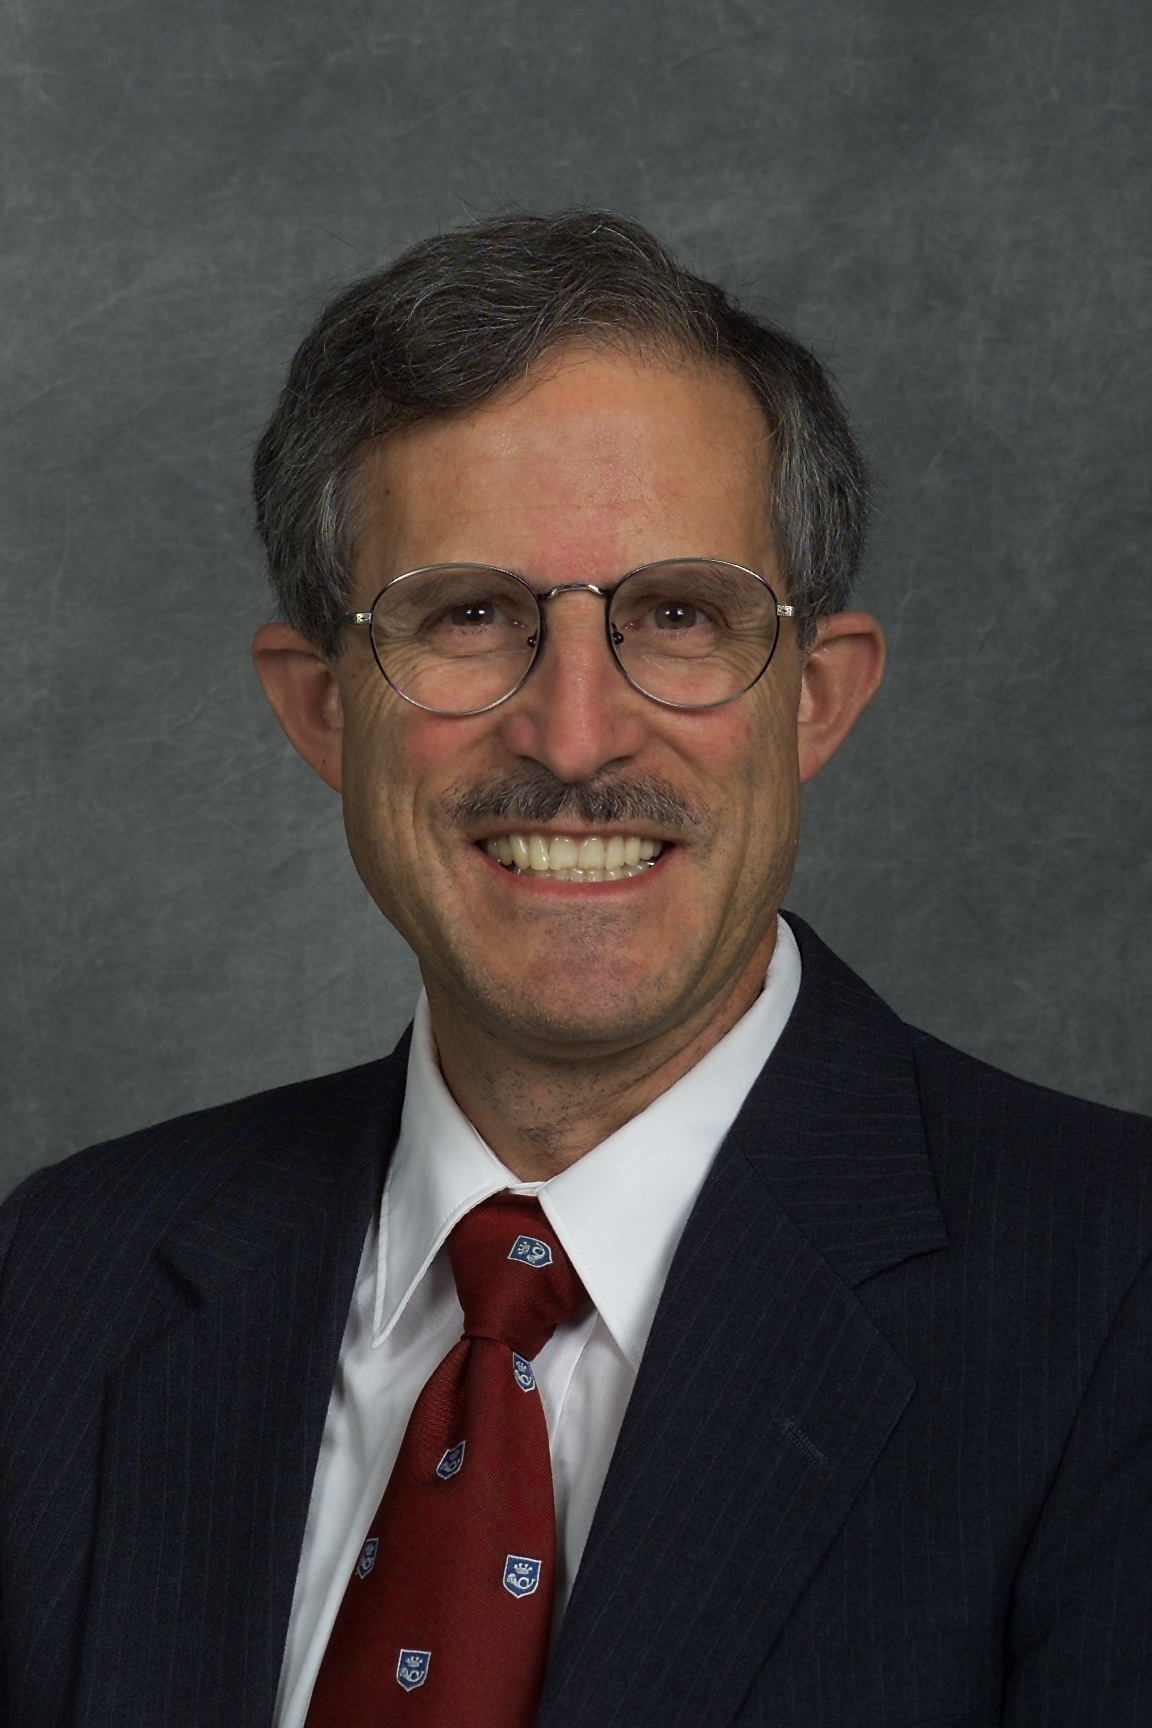
\includegraphics[height=5.3cm]{Day1/images/dhb.jpg}}
\end{column}
\end{columns}

\end{frame}


\subsubsection{The choice of the (right) compiler}

\begin{frame}[containsverbatim]
\frametitle{The compiler issue}
\label{compilerissue}
\begin{block}{}
The choice of the compiler is \textbf{very} important. Different version can lead to different performance on the same code.
\end{block}

\begin{lstlisting}[language=C,frame=lines]
      for (i=0;i<N;i++){
         for (j=0;j<N;j++){
            for (k=0;k<N;k++){
               C[i][j]=C[i][j] + A[i][k]*B[k][j];
            }
         }
      }
\end{lstlisting}

\begin{block}{}
We change the loop order and the compiler version: \texttt{i-j-k}, \texttt{i-k-j}, \texttt{j-i-k}, \texttt{j-k-i}, \texttt{k-i-j}, \texttt{k-j-i} and the two compilers: \texttt{gcc-4.8.2}, \texttt{icc 15}.
\end{block}

\end{frame}

\begin{frame}[containsverbatim]
\frametitle{\texttt{gcc} version 4.8.2, N=2000}

\verb+gcc -O3 -ftree-vectorize dgemm.c -lgsl + \\
\verb+    -lblas -lm -o dgemm+

%\begin{verbatim}
%  ijk    8000000000.00000     83.4875031      [MF/s]
%  ikj    8000000000.00000     1384.72632      [MF/s]
%  jik    8000000000.00000     83.6547699      [MF/s]
%  jki    8000000000.00000     191.552567      [MF/s]
%  kij    8000000000.00000     1517.48328      [MF/s]
%  kji    8000000000.00000     183.618088      [MF/s]
%  MKL    8000000000.00000     10047.3174      [MF/s]
%\end{verbatim}

\begin{verbatim}
  ijk         0.133   [GF/s]
  ikj         2.128   [GF/s]
  jik         0.132   [GF/s]
  jki         0.064   [GF/s]
  kij         1.914   [GF/s]
  kji         0.064   [GF/s]
  DGEMM OPT   10.35   [GF/s]
\end{verbatim}


\begin{block}{Remark}
``DGEMM OPT'' stands for the ATLAS library
\end{block}
\end{frame}

\begin{frame}[containsverbatim]
\frametitle{\texttt{icc} version 15, N=2000}

\verb+icc -DMKL_IN_USE -DMKL_ILP64 -openmp -I${MKLROOT}/include +\\
\verb+    -O3 -xHost dgemm.c  -L${MKLROOT}/lib/intel64 +\\
\verb+    -lmkl_intel_ilp64 -lmkl_core -lmkl_intel_thread+\\
\verb+    -lpthread -lm -o dgemm+

%\begin{verbatim}
%  ijk    8000000000.00000        6061.952      [MF/s]
%  ikj    8000000000.00000        6554.129      [MF/s]
%  jik    8000000000.00000        6001.980      [MF/s]
%  jki    8000000000.00000        6448.704      [MF/s]
%  kij    8000000000.00000        1636.432      [MF/s]
%  kji    8000000000.00000        6580.376      [MF/s]
%  MKL    8000000000.00000        10031.17      [MF/s]
%\end{verbatim}

\begin{verbatim}
  ijk         2.746   [GF/s]
  ikj         2.784   [GF/s]
  jik         2.586   [GF/s]
  jki        10.233   [GF/s]
  kij         2.747   [GF/s]
  kji         9.815   [GF/s]
  DGEMM OPT  27.593   [GF/s]
\end{verbatim}

\begin{block}{Remark}
``DGEMM OPT'' stands for the Intel Math Kernel Library (version 11.2)  on 8 cores
\end{block}
\end{frame}


\begin{frame}[containsverbatim]
	\frametitle{Optimization. Always ?}

Is it possible to optimize the following loop :

\begin{lstlisting}[language=Fortran,frame=lines]
do i=1,N
   do j=1,N
     y(i) = y(i) + alpha*A(i,j)*x(i) + beta*y(i)
   enddo
enddo
\end{lstlisting}

$y = \alpha A x + \beta y$

\end{frame}

\begin{frame}[containsverbatim]
	\frametitle{Optimization. Always ?}

%\begin{table}
\begin{center}
\begin{tabular}{|l|l|l|l|}
\hline
 \textbf{OPTIMIZATION} & \textbf{time (gcc)} & \textbf{time (icc)} & Difficulty \\
\hline
\hline
None ({\tt -O0}) & 65.4 & 74.1 & \\
\hline
Compiler ({\tt -O3}) & 38.6 & 1.73 & really easy\\
\hline
Compiler ({\tt -O3} + SIMD) & 39.34 & 2.6 & really easy\\
\hline
By hands (loop change) & 2.33 & 2.2 & can be compl.\\
\hline
External lib$^1$ & 0.72 & 0.70 & easy\\
\hline
\end{tabular}
\end{center}
%\caption{\texttt{N=40000}, time is in seconds. $^1$  call to dgemv() in libblas}
\texttt{N=40000}, time is in seconds. $^1$  call to dgemv() in libblas
%\end{table}

\end{frame}


\begin{frame}
	\frametitle{Performance}

{\bf Flop} (Floating Point Operations per Second)

	\begin{itemize}
	\item MFlops = MF = MF/s (MegaFlops), GFlops = GF = GF/s (GigaFlops), etc ..
	\item How to measure the Flops ?
		\begin{itemize}
			\item by hand (theoretical number of operations devided by the running time)
			\item with external tools (all based on hardware counters) : PAPI, Tau, likwid, Intel Amplxe, etc..
		\end{itemize}
	\end{itemize}

{\bf Memory} Memory Bandwidth and Memory latency

	\begin{itemize}
	\item Bandwidth in Bytes per second, latency in seconds (micro-second)
	\item How to measure memory characteristics
		\begin{itemize}
			\item by hand (theoretical number of accesses devided by the running time)
			\item with external tools (all based on hardware counters) : PAPI, Tau, Intel Amplxe, etc..
		\end{itemize}
	\end{itemize}
\end{frame}


\begin{frame}[containsverbatim]
	\frametitle{Performance example}

\begin{lstlisting}[language=C,frame=lines]
   struct timeval t;
   double t1 = gettimeoftheday(&t,0);
      for (i=0;i<N;i++){
         for (j=0;j<N;j++){
            for (k=0;k<N;k++){
               C[i][j]=C[i][j] + A[i][k]*B[k][j];
            }
         }
      }
   double t2 = gettimeoftheday(&t,0);
   double mflops = 2.0*pow(N,3) / (t2-t1) / 1.0E6 ;
\end{lstlisting}

$2 N^3$ operations

\end{frame}


